\documentclass{beamer}
\usepackage[english]{babel}
\usepackage[utf8]{inputenc}
\usepackage{beamerthemesplit}
\usepackage{graphics,epsfig, subfigure}
\usepackage{url}

\definecolor{WISblue}{RGB}{69,91,168}

\setbeamercovered{transparent}
\mode<presentation>
{  \usetheme{PaloAlto}
  \usecolortheme[named=WISblue]{structure}
  \useinnertheme{circles}
  \usefonttheme[onlymath]{serif}
  \setbeamercovered{transparent}
  \setbeamertemplate{blocks}[rounded][shadow=true]
}

\logo{
\includegraphics[width=1.3cm]{figs/logo}}


\title{Kupcinet-Getz Summer School Project}
\subtitle{Optimising Polymer Layer for use in Schottky-type silicon solar cells}
\author{Timo Bretten}
\institute{Weizmann Institute of Science \\ Rehovot, Israel}
\date{\today}

\begin{document}

\frame{
\titlepage \vspace{-0.5cm}
\begin{center}
%
\includegraphics[height=0.25\textheight]{figs/logo}
\end{center}
}

\frame{
\frametitle{Layout}
\tableofcontents[pausesection]
}

\section{Introduction}
\frame{
\frametitle{Solar pros and cons}
\begin{center}
\begin{block}{Solar Cells can be}
\begin{columns}
\column{.3\textwidth} \hspace{0.5cm}
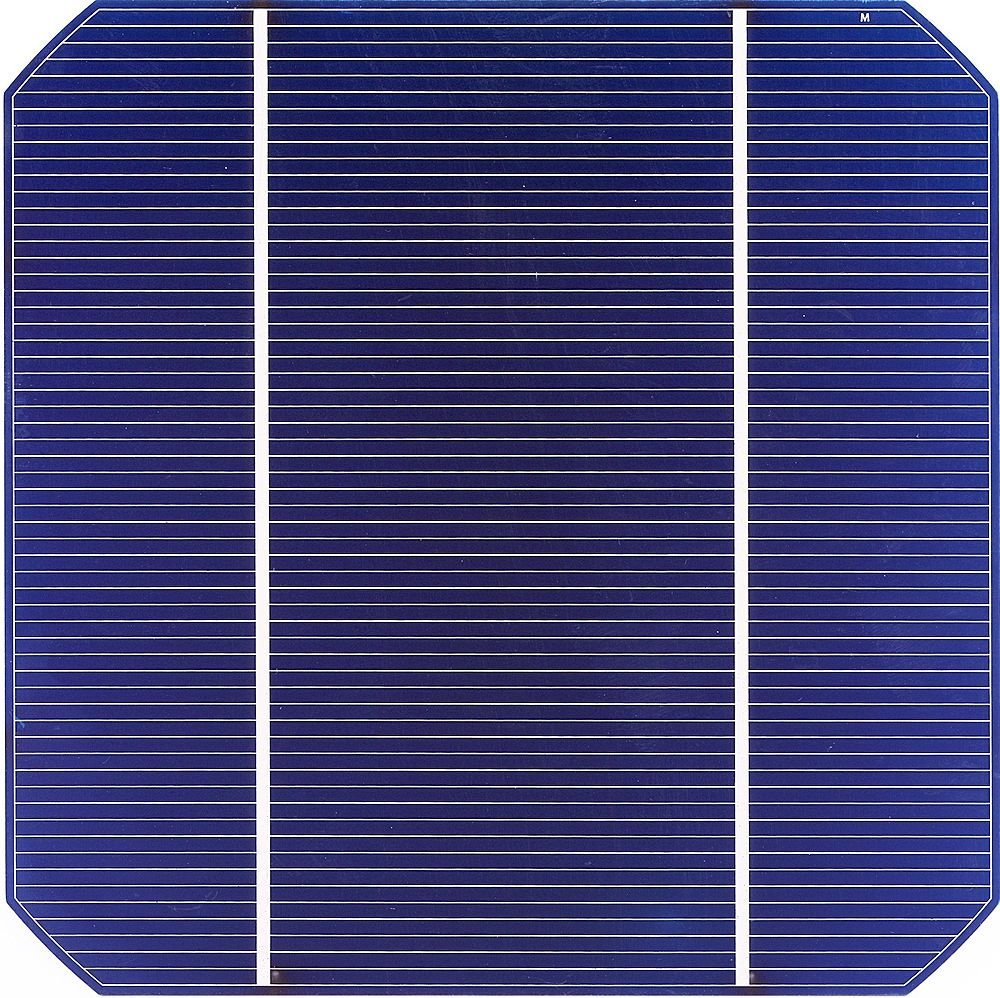
\includegraphics[width=0.7\textwidth]{figs/si} 
\column{.7\textwidth}
\begin{itemize}
\item Very efficient
\pause
\item Very sustainable
\pause
\item Quite costly
\end{itemize}
\end{columns}
\end{block}
\visible<1->{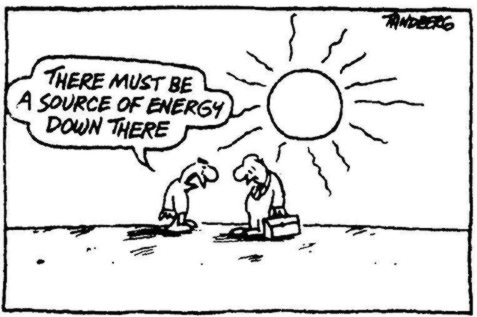
\includegraphics[width=6cm]{figs/mustbe}}
\end{center}
}

\subsection{Schottky-type solar cells}
\frame{
\frametitle{Achieving Conversion}
\begin{block}{Generic Block, with columns}
\begin{columns}
\column{.3\textwidth} \hspace{0.5cm}
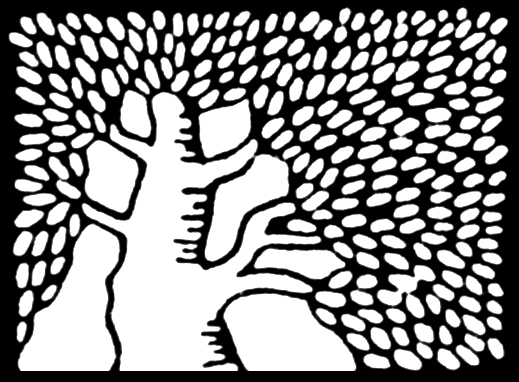
\includegraphics[width=0.7\textwidth]{figs/logo_bw} 
\column{.7\textwidth}
Block with fig and text
\end{columns}
\end{block}
}
\subsection{PDOT:PSS}
\frame{
\frametitle{A (poorly) conductive polymer}
\begin{block}{Generic Block, with columns}
\begin{columns}
\column{.3\textwidth} \hspace{0.5cm}
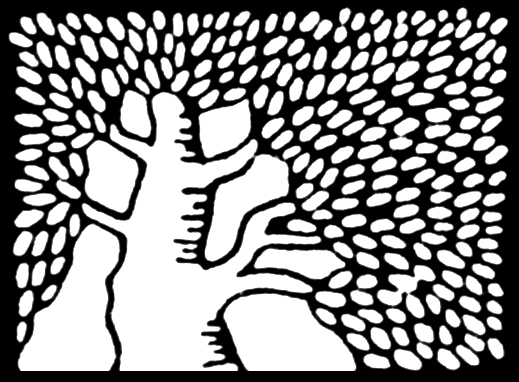
\includegraphics[width=0.7\textwidth]{figs/logo_bw} 
\column{.7\textwidth}
Block with fig and text
\end{columns}
\end{block}
}

\section{Experimental...}
\subsection{...Procedure}
\frame{
\uncover<1>{
\frametitle{Making films and devices}
\begin{block}{Workflow for films}
\begin{itemize}
\item Clean glass plates
\item Mix desired polymer solution
\item Spin-coat solution on glass \& anneal
\end{itemize}
\end{block}
}
\uncover<2>{
\begin{block}{Workflow for devices}
\begin{itemize}
\item Make films as before
\item Clean silicon
\item Lift-off film from glass then float on film to silicon \& anneal
\item Evaporate Ag top-contact to Si
\end{itemize}
\end{block}
}
}

\frame{
\frametitle{Characterising films and decives}
\uncover<1>{
\begin{block}{Workflow for films}
\begin{itemize}
\item Use 4-point probe to measure resistance
\item Use spectrometer to measure transmittance
\item Use AFM to find film thickness
\item Convert resistance to resistivity \& transmittance to transmissivity
\end{itemize}
\end{block}
}
\uncover<2>{
\begin{block}{Workflow for devices}
\begin{itemize}
\item Measure J-V
\item Measure cell area
\item Find efficiency $\eta$ and fill-factor
\end{itemize}
\end{block}}
}

\subsection{...Results}
\frame{
\frametitle{Resistivity} 
} 

\frame{
\frametitle{Transmissivity}
}

\frame{
\frametitle{Device Performance}
}

\section{Conclusion}

\frame{
\frametitle{In a nutshell}
\begin{columns}
\column{0.3\textwidth}{
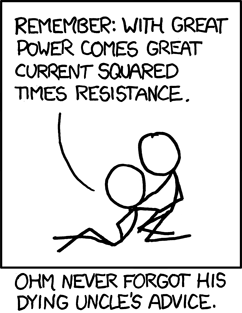
\includegraphics[width=1\textwidth]{figs/ohm}
}
\column{0.7\textwidth}{
\begin{itemize}
\item PDOT:PSS properties could be optimised
\item I learned a lot about solar cells, especially lab skills
\pause
\item We had a great time
\end{itemize}
}
\end{columns}
}


\section{References and Thanks}
\frame{
\frametitle{I would like to thank}
\begin{block}{Prof. David Cahen}
\begin{columns}
\column{0.35\textwidth}{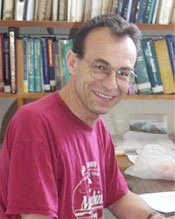
\includegraphics[height=0.9\textwidth]{figs/david}}
\column{0.55\textwidth}{Professor David Cahen for accepting me into his group}
\end{columns}
\end{block}}

\frame{
\frametitle{I would like to thank}
\begin{block}{Dr. Ann Erickson}
\begin{columns}
\column{0.35\textwidth}{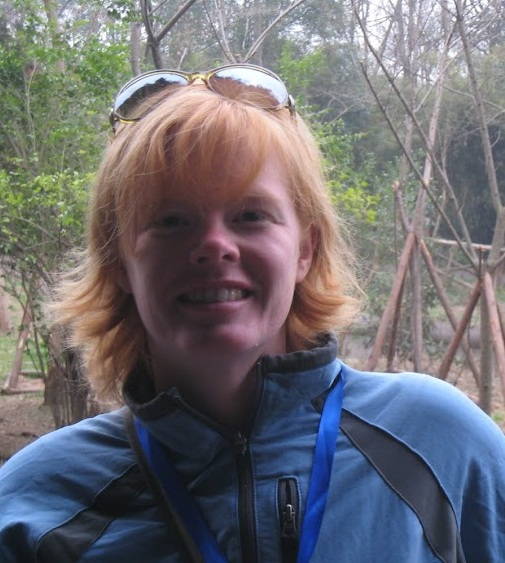
\includegraphics[width=0.9\textwidth]{figs/ann}}
\column{0.55\textwidth}{Doctor Ann ``Super-Ann''  Erickson for sharing her wisdom and skills}
\end{columns}
\end{block}}

\frame{
\frametitle{I would like to thank}
\begin{block}{Lior}
\begin{columns}
\column{0.35\textwidth}{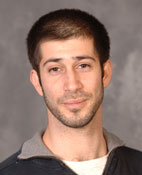
\includegraphics[width=0.9\textwidth]{figs/lior}}
\column{0.55\textwidth}{Lior Sepunaro for undoubtedly the best espresso ever}
\end{columns}
\end{block}}

\frame{
\frametitle{This project is based on work by}
\tiny
\begin{itemize}
\item Thomas R. N. Jansson, Martin P. Haspang, Kåre H. Jensen, Pascal Hersen, and Tomas Bohr,
\textit{Polygons on a Rotating Fluid Surface}, Physical Review Letters \textbf{96}, 174502 (2006) 
 \item Vatistas, G.H., "A Note on Liquid Vortex Sloshing and Kelvin's
Equilibria", JFM, vol. 217, 1990, p. 241.
\item Vatistas, G. H., Wang, J., and Lin, S. "Experiments on Waves Induced
in the Hollow Core of Vortices". J. Exp. Fluids, vol 13, 1992, p.377.
\item Vatistas, G. H., Wang, J., and Lin, S. "Recent Findings on Kelvin's
Equilibria", Acta Mechanica, vol. 103, 1994, p. 89.
\item Vatistas, G.H., Esmail, N., and Ravanis, C. "Wave Development in
Disk-Like Nearly Inviscid Liquid Vortices", 39th AIAA Aerospace Sciences
Meeting and Exhibit. Paper no. AIAA 2001-0168, 8-11 January 2001, Reno, NV.
\end{itemize}
}


\end{document}
